\documentclass[11pt,a4paper]{article}
\usepackage{fontspec}
\setmainfont{TeX Gyre Pagella}
\newfontfamily\headfont{Inter}[UprightFont=*-ExtraBold,BoldFont=*-ExtraBold,Extension=.otf,Path=/usr/share/fonts/opentype/inter/]
\usepackage[a4paper,margin=2.3cm]{geometry}
\usepackage{graphicx,booktabs,float,caption,array,xcolor,longtable}
\usepackage{xurl}
\usepackage[hidelinks]{hyperref}
\usepackage{titlesec}
\usepackage[round]{natbib}
\usepackage{setspace}
\setstretch{1.05}
\renewcommand{\topfraction}{0.9}
\renewcommand{\bottomfraction}{0.8}
\renewcommand{\textfraction}{0.1}
\renewcommand{\floatpagefraction}{0.75}
\setlength{\parindent}{0pt}
\setlength{\parskip}{0.55em}
\titleformat{\section}{\headfont\Large}{\thesection}{0.8em}{}
\titleformat{\subsection}{\headfont\large}{\thesubsection}{0.8em}{}
\captionsetup{font=small,labelfont=bf}
\urlstyle{same}
\hypersetup{pdftitle={The World According to the Hereford Mappa Mundi},pdfauthor={Tristan Hotham}}

\begin{document}
\begin{center}
{\Large\bfseries The World According to the Hereford Mappa Mundi\par}
\vspace{0.4em}
{\large A medieval map of the world set against a modern one:\\the 1,025 names of Bevan and Phillott's index, identified, classified and measured\par}
\vspace{1.2em}
{\large Tristan Hotham\par}
\vspace{0.3em}
{\small Independent researcher\\
ORCID: 0000-0003-4931-9349\\
DOI: https://doi.org/10.5281/zenodo.23878612\par}
\vspace{0.8em}
2026
\end{center}

\begin{quote}
\small
\begin{center}\textbf{Abstract}\end{center}
The Hereford Mappa Mundi (about 1300) is the largest surviving medieval map of the world. I use the index of names compiled by Bevan and Phillott in 1873 as an inventory of the map (1,025 names), assign each to the four kinds of material those authors distinguished, and compare the positions of 164 inscriptions, located by eye on Konrad Miller's 1896 facsimile, with the real places the 1873 book identifies. Of the 985 names that are not part of the map's frame or natural history, 72\% are classical, 9\% Biblical, 12\% medieval and 6\% legendary; every Biblical name is in Asia, and 92\% of the names in the British Isles are medieval. Britain and Ireland, 0.4\% of the land of Africa, Asia and Europe, carry 8.1\% of the names. Measured from Jerusalem, the map's centre, directions are kept well once east is put at the top: the median error for the 140 located real places is 19 degrees and 81\% lie within 45 degrees. Distances are kept in order (rank correlation 0.90) but compressed towards the rim: places a median 3,747 km away are only 4.8 times as far out on the map as places a median 128 km away. Relative to the map as a whole, the Holy Land is drawn 4.5 times larger, the British Isles 1.5 times, and India and Central Asia at 0.71 of the average. The map spends its space on Scripture and on home.

\textbf{Keywords:} medieval cartography; mappa mundi; Hereford; historical geography; map distortion; Pleiades; open data
\end{quote}

\section{Introduction}
The Hereford Mappa Mundi, drawn on a single sheet of vellum about 158 by 133 cm and kept in Hereford Cathedral, is the largest medieval map of the world known to survive \citep{wiki}. It follows the T and O pattern: the inhabited world is a disc ringed by ocean, with east at the top, Jerusalem at the centre, Asia filling the upper half and Europe and Africa the lower quarters, divided by the Mediterranean, the Don and the Nile. It is a religious and encyclopedic object rather than a guide for travellers, and it mixes Biblical history, classical geography, the marvels of the Alexander romance and a detailed picture of the mapmaker's own island.

Bevan and Phillott's \textit{Mediaeval Geography} \citep{bevan} went over the map name by name, region by region, identifying each name where they could and tracing it to its source, and ended with an index of names. That index, and the scanned text of the book, are the core of this study. I ask four questions. How many names does the map carry, and in which parts of the world? What share is Biblical, classical, medieval and legendary? Which real places did it include? And how distorted is it, in direction, in distance and in the space it gives to each region? The paper accompanies an interactive comparison of the map and a modern map (\url{https://maps.tristanhotham.com/mappa-mundi/}).

\section{Data}
\textbf{The book.} The Internet Archive's scan of \citet{bevan} (public domain) provides the text, divided here into the book's 174 pages using the running heads. The book's chapters follow the map: the frame and the ocean (chapter I), Asia (II to IV), Africa (V), the Mediterranean and Black Sea with their islands (VI), Europe (VII and VIII) and the British Isles (IX). The map's own words are printed in black-letter type, which the OCR renders as nonsense; the commentary, identifications and citations are in roman type and read cleanly. Miller's \textit{Die Herefordkarte} \citep{miller1903} was used for cross-checks.

\textbf{The images.} Konrad Miller's 1896 facsimile \citep{miller1896}, a hand-drawn copy with clear labels (3,840 by 4,708 pixels as used), and a photograph of the original (Wikimedia Commons, an enlargement of a 600 pixel image, so its labels cannot be read). Both are in the public domain.

\textbf{Gazetteers.} Pleiades, a gazetteer of ancient places \citep{pleiades}, version 4.1, and Natural Earth countries and towns \citep{naturalearth}. Facts on the map's size, date and contents are from English Wikipedia \citep{wiki}.

\section{Methods}
\subsection{Inventory}
The book's index, ``Index of the names of places and objects [on the] Hereford Mappa Mundi'', has 1,025 entries once lines broken by the scan are rejoined, each with a type where given (river, island, mountain, sea, promontory, gulf) and the page or pages that discuss it. I corrected OCR errors in the index names (rn read as m, N as K, and so on) and in ten page numbers, checking each against the text. The part of the world is that of the chapter the first page falls in. The index records names, not pictures: a town with a label is one entry, an unlabelled picture is none, and some legends are indexed under their key word.

\subsection{Classes}
Bevan and Phillott sort the map's materials into Biblical, classical, legendary and contemporaneous (medieval) \citep[Introduction, section 11]{bevan}. I applied that scheme with a fixed rule, in order. (1) The winds, quarters and continent labels of the frame and the real animals and plants (40 names) are left out. (2) Legendary: monstrous peoples, fabulous beasts, and the places and objects of legend and myth, from a list drawn up name by name. (3) Biblical: every name in the book's sections on the rivers of Paradise (pp. 25 to 26), Palestine and Arabia (pp. 77 to 81) and the Exodus in Egypt (pp. 85 to 86), less the Greek and Roman names there, and a few Biblical names elsewhere (Babel, Babylon, Ur, Nineveh, Noah's Ark, Enos, Ophir). (4) Medieval: in the British Isles every name except five from Roman writers; in the rest of Europe a list of post-Roman places, regions and peoples; in Asia and Africa only six names of medieval origin (Samarkand, the Turks, the monasteries of St Antony, St Zosimas and Mahun). (5) Classical: everything else. The lists are in the published code.

\subsection{Real places}
For each inscription I located on the facsimile (below) I read the book's identification and recorded it with the page and the book's words, and gave the modern place's coordinates, checked against Natural Earth. For the other names I looked for the same name in Pleiades (attested and romanised names and place titles), allowing simple medieval spellings (y for i, f for ph, ablative endings), within a box for the part of the world the book discusses the name under; approximate spellings were allowed with a similarity of at least 0.86 and the same first two letters. Every match was checked by hand against the part of the world the book puts the name in and the place it points to; 78 that pointed to another place of the same or a similar name were rejected. In all 337 of the 928 names that are neither frame nor legend (36\%) have a real position: 143 from the book and 194 from Pleiades (32 of them with rough Pleiades locations). This is a lower bound on what can be identified.

\subsection{Positions on the map}
No coordinate dataset exists for the Hereford map, so I located 164 well-known and legible inscriptions by eye on the facsimile, at the town picture or, where there is none, at the middle of the label, recording my confidence (119 read clearly, 45 with some doubt because the label is worn, crowded or ambiguous). Of these, 16 are legendary and 143 are identified with a real place (140 distinct places once Babel and Babylon, and Santiago and its shrine, are merged). Positions were carried to the photograph by an affine fit on 9 features clear on both images (Jerusalem, Paradise, the Pillars of Hercules, the Tower of Babel, Delos, Crete, Charybdis, the Well of the Sun and Lake Salinarum), with a root mean square error of 44 pixels, about 1.4\% of the map's width.

\subsection{Distortion}
For each located real place I measured the true great-circle distance and initial bearing from Jerusalem (31.78 N, 35.23 E) and the distance and bearing on the facsimile from the centre of the walled circle of Jerusalem, reading east as up. Map distance is expressed as a share of the map radius, the mean distance from Jerusalem to Paradise and to the Pillars of Hercules (1,536 pixels). To summarise the scale of each region, I took all pairs of located places in the region at least 100 km apart and computed the median of map distance over true distance, divided by the same median over all such pairs on the map; regions with fewer than five located places are not scored. Finally, I fitted the similarity transform (rotation, uniform scale and shift, least squares) that best lays the located map positions on an azimuthal equidistant projection centred on Jerusalem, and measured each place's displacement from where that fit puts it.

\section{Results}
\subsection{What is on the map}
Table~\ref{tab:parts} and Figure~\ref{fig:parts} show the inventory. Asia has 371 names, Europe 324, Africa 117, the seas and islands 105 and the British Isles 83. 640 are settlements, regions or peoples, 139 rivers, 108 islands and 69 mountains. For comparison, Wikipedia counts about 420 towns, 15 Biblical events, 33 animals and plants, 32 people and 5 scenes from classical mythology \citep{wiki}.

\begin{table}[tbp]\centering\small\caption{Names in Bevan and Phillott's index by part of the map and class (frame and natural history left out).}\label{tab:parts}\begin{tabular}{lrrrrr}\toprule Part of the map & Names & Biblical & Classical & Medieval & Legendary\\\midrule
Asia & 360 & 93 & 225 & 6 & 36\\
Africa & 114 & 0 & 103 & 0 & 11\\
Europe & 321 & 0 & 279 & 39 & 3\\
British Isles & 83 & 0 & 5 & 76 & 2\\
Seas and islands & 105 & 0 & 100 & 0 & 5\\
\midrule All & 985 & 93 & 714 & 121 & 57\\
\bottomrule\end{tabular}\end{table}

\begin{figure}[tbp]\centering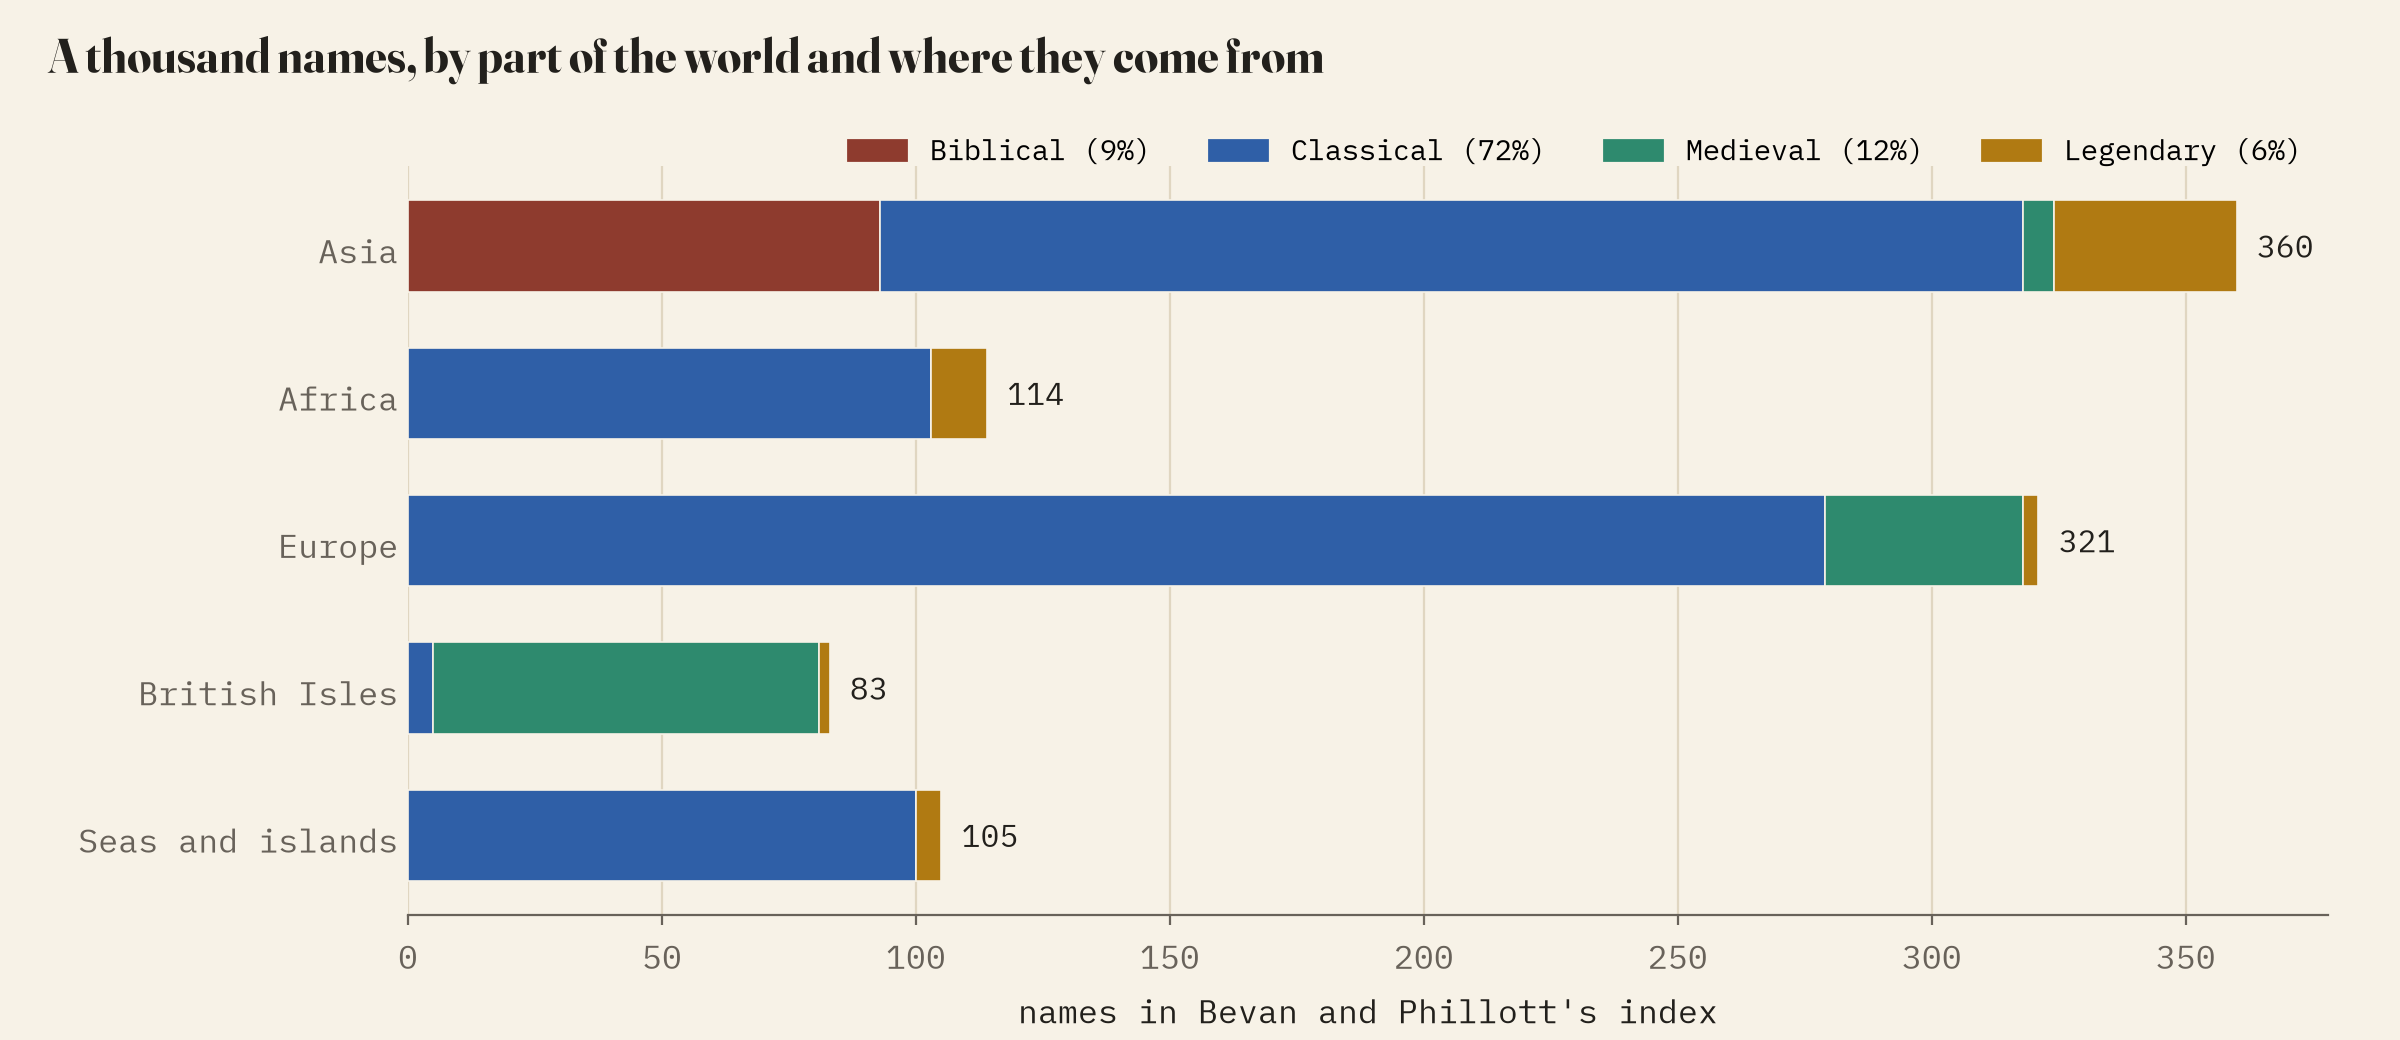
\includegraphics[width=\textwidth]{f_parts.png}
\caption{Names in Bevan and Phillott's index by part of the map and class.}\label{fig:parts}\end{figure}

By the rule above, 714 names (72\%) are classical, 93 (9\%) Biblical, 121 (12\%) medieval and 57 (6\%) legendary. All 93 Biblical names are in Asia, as are 36 of the legendary ones. Africa's names are 90\% classical, Europe's 87\%. The British Isles are the exception, 92\% medieval, consistent with Bevan and Phillott's remark that the mapmaker's contemporary knowledge is ``almost entirely confined to Europe'' and with the detail of the British section.

\subsection{Real places and their positions}
Figure~\ref{fig:maps} shows the located inscriptions on the facsimile and the identified places on a modern map; Appendix Table~\ref{tab:located} lists them.

\begin{figure}[tbp]\centering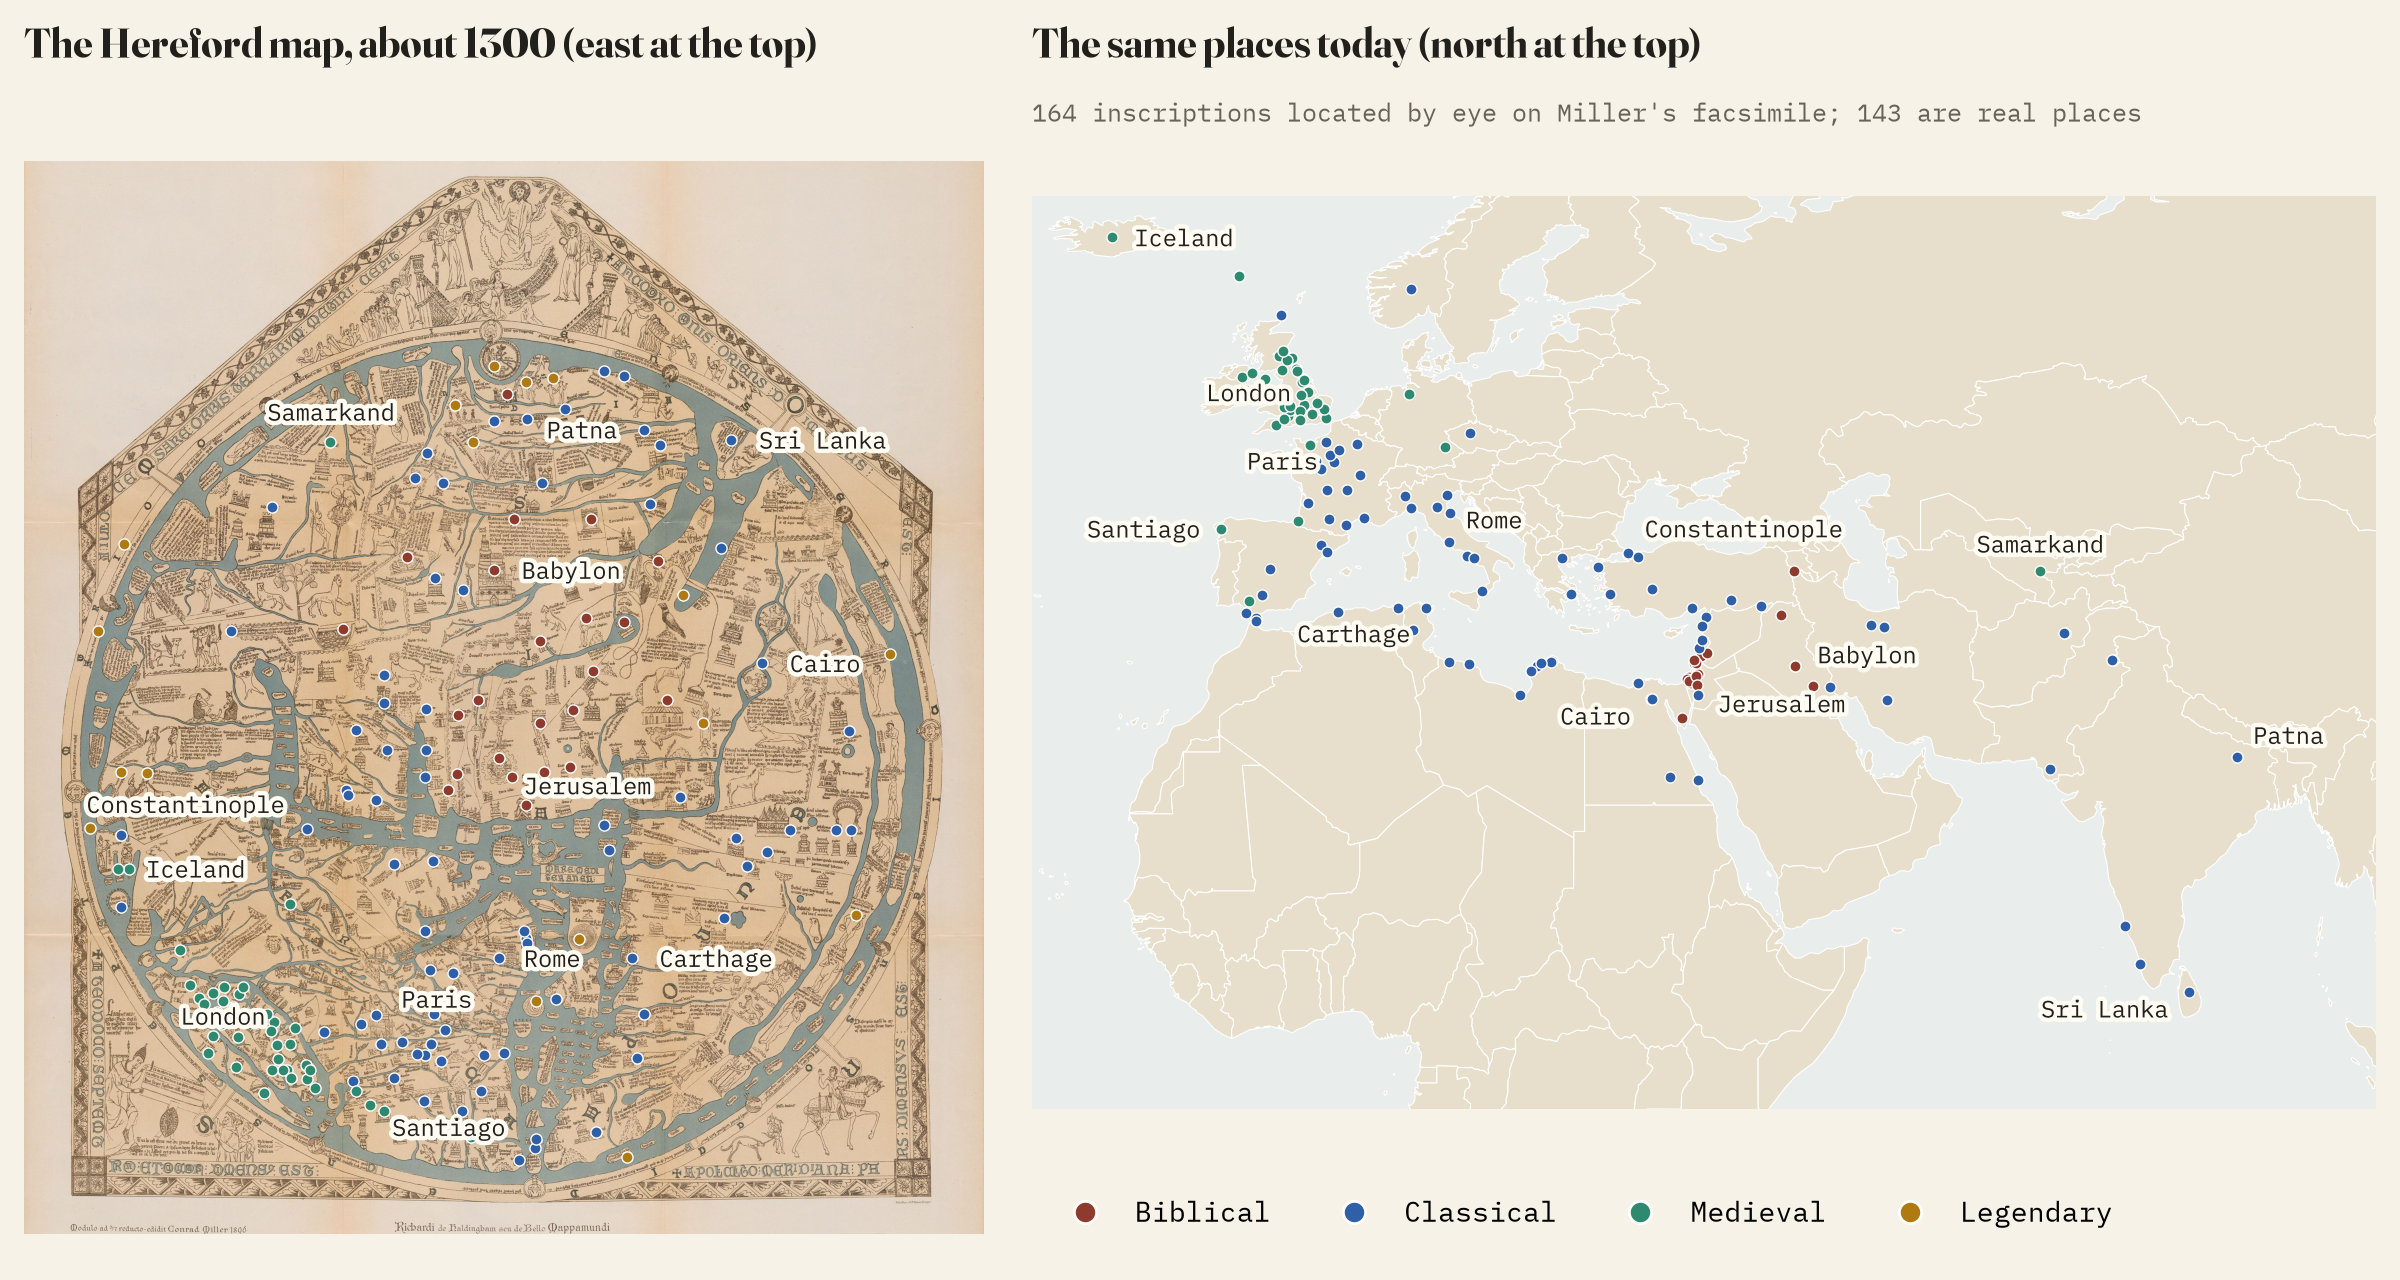
\includegraphics[width=\textwidth]{f_maps.png}
\caption{Located inscriptions on Miller's facsimile (left, east at the top) and the places the 1873 book identifies, on a modern map (right). Colours are classes.}\label{fig:maps}\end{figure}

\subsection{Direction}
Bearings from Jerusalem are kept well (Figure~\ref{fig:bearing}). The median absolute error is 19 degrees, 81\% of places are within 45 degrees and all are within 90. The errors are not random: North Africa (69 degrees) and Egypt (72) are swung southward, because the Mediterranean is drawn as a straight channel from the Pillars of Hercules at the bottom of the map to the Holy Land at its centre, while the British Isles (8), Mesopotamia and Persia (12) and India and Central Asia (10) point close to the right way. The best-fitting rotation turns the map's top to a bearing of 98 degrees, a little south of due east, and explains 0.84 of the variance of the true positions; the median displacement from the fitted position is 516 km (Figure~\ref{fig:arrows}).

\begin{figure}[tbp]\centering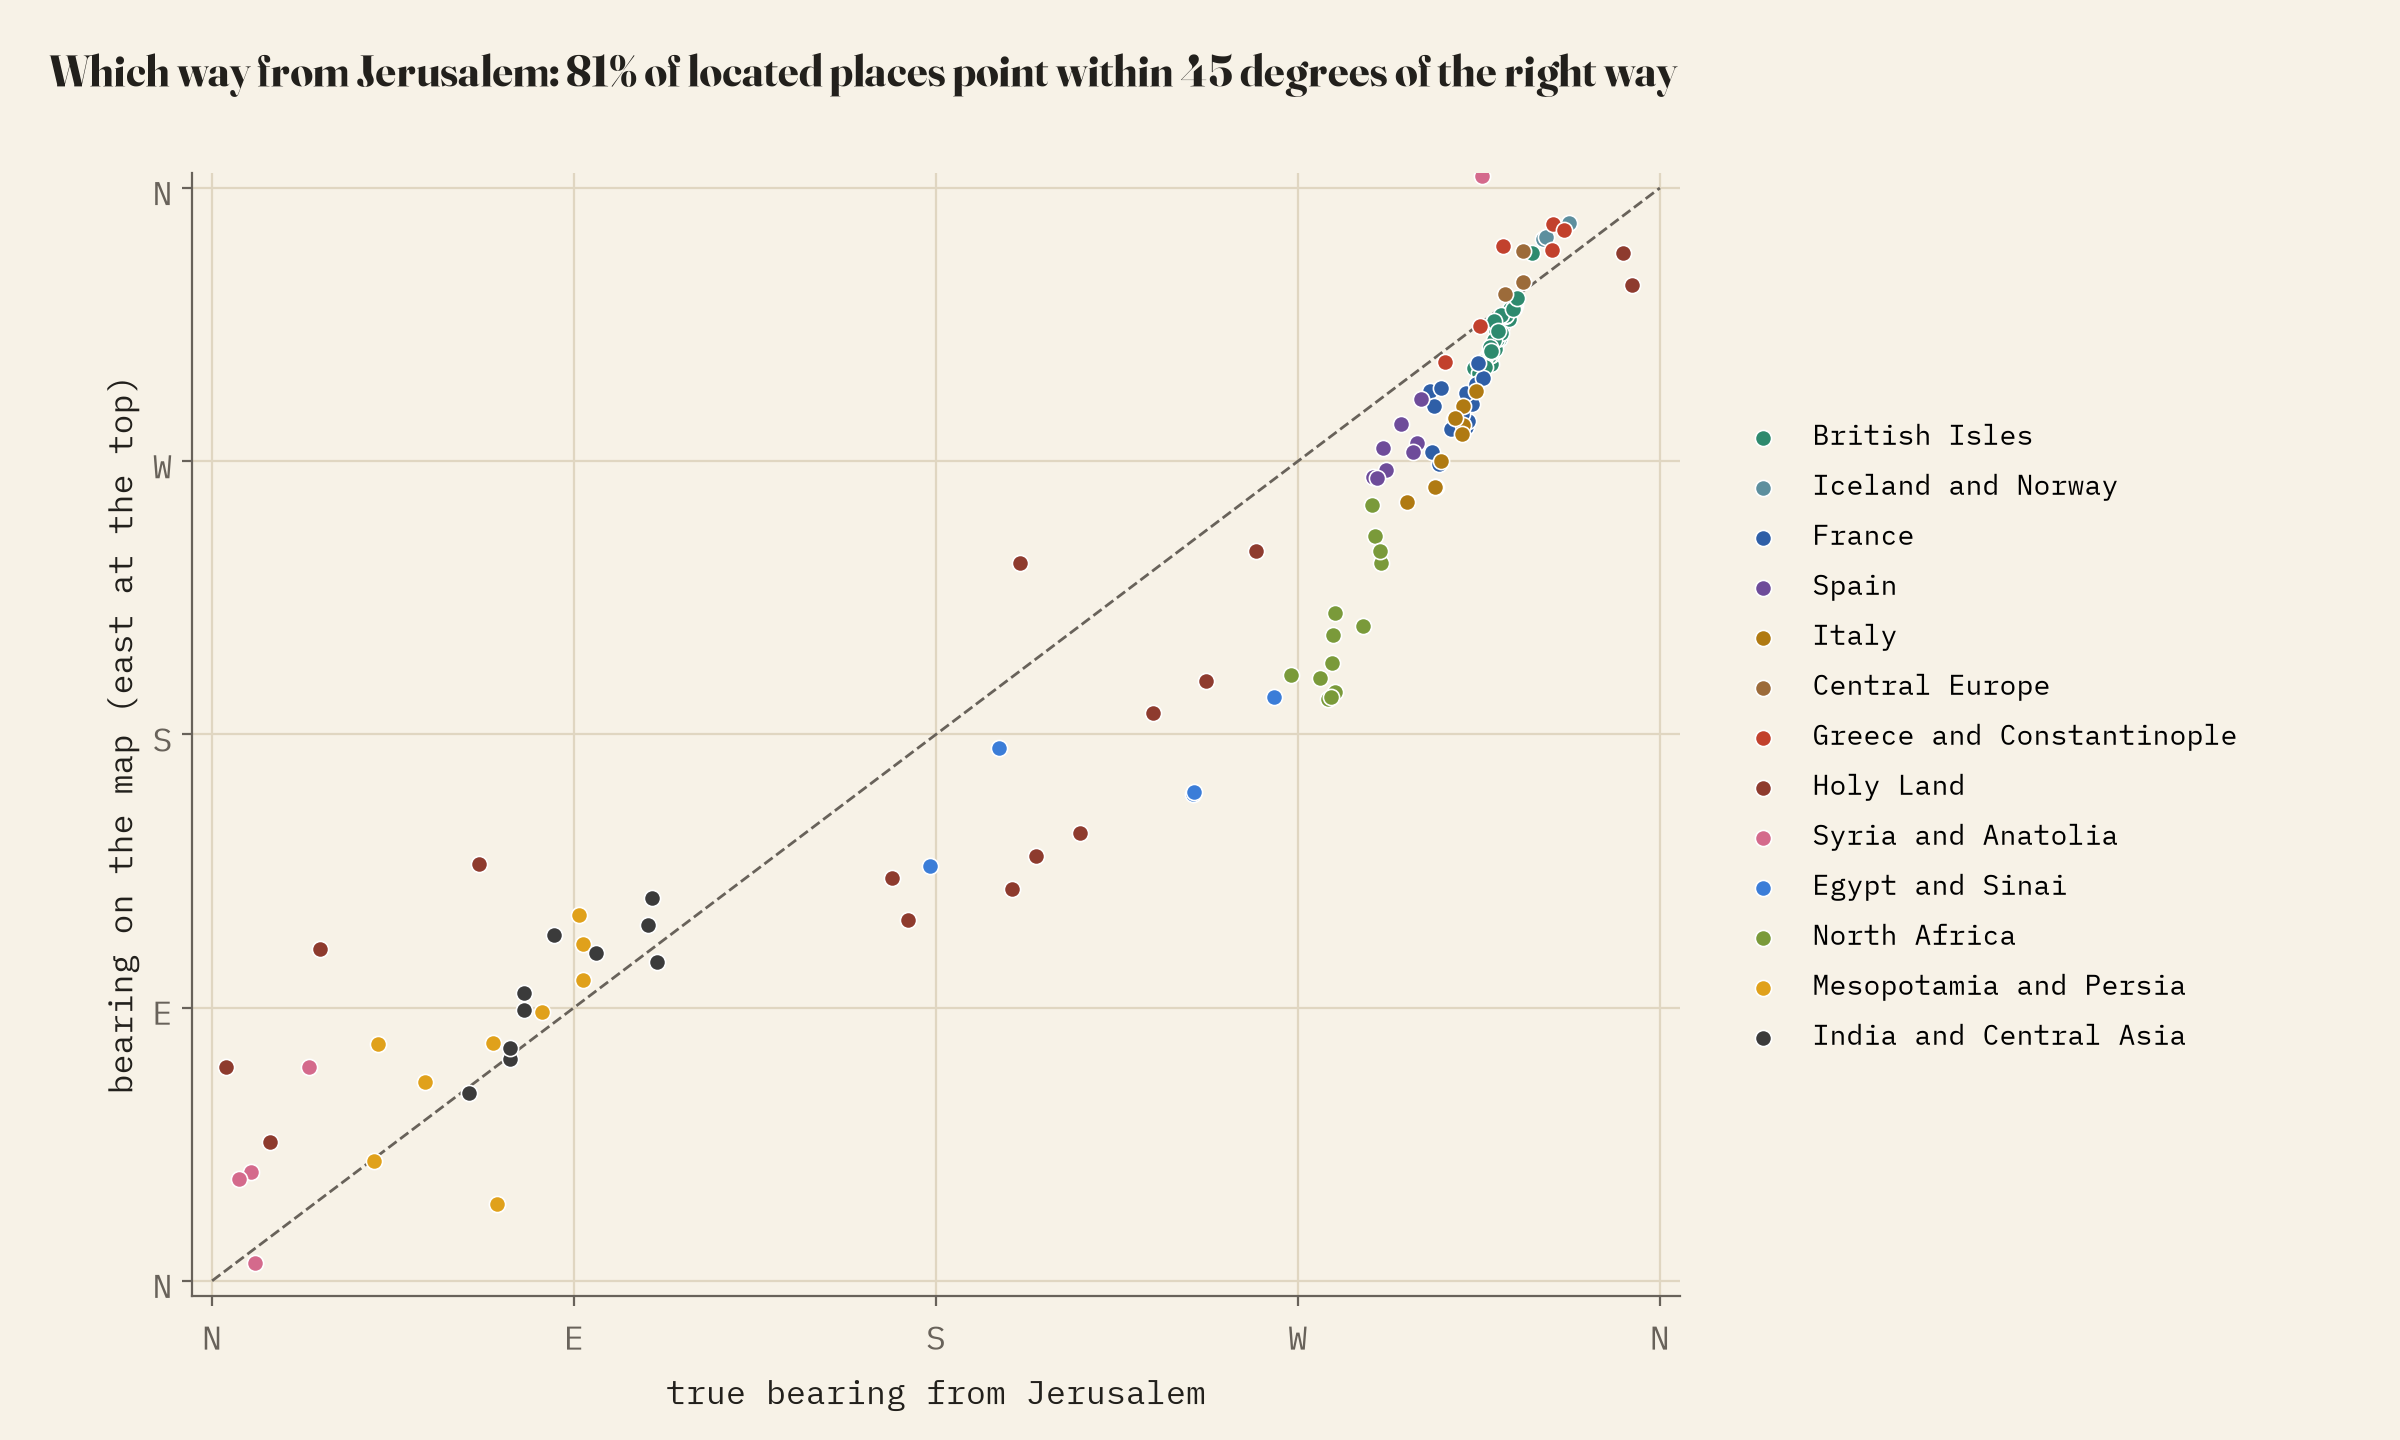
\includegraphics[width=\textwidth]{f_bearing.png}
\caption{Bearing from Jerusalem on the map (east up) against the true bearing, by region. The dashed line is perfect agreement.}\label{fig:bearing}\end{figure}

\subsection{Distance}
Distances keep their order (Spearman's rank correlation 0.90) but not their scale (Figure~\ref{fig:distance}). Places within 500 km of Jerusalem (median 128 km) sit a median 20\% of the way to the rim; places 3,000 km or more away (median 3,747 km) sit at 93\%: 29.3 times as far in reality, 4.8 times on the map. Bethlehem, 9 km from Jerusalem, is 6\% of the way out; London, 401 times farther, is at 90\%; Sri Lanka, 5,398 km away, sits on the rim.

\begin{figure}[tbp]\centering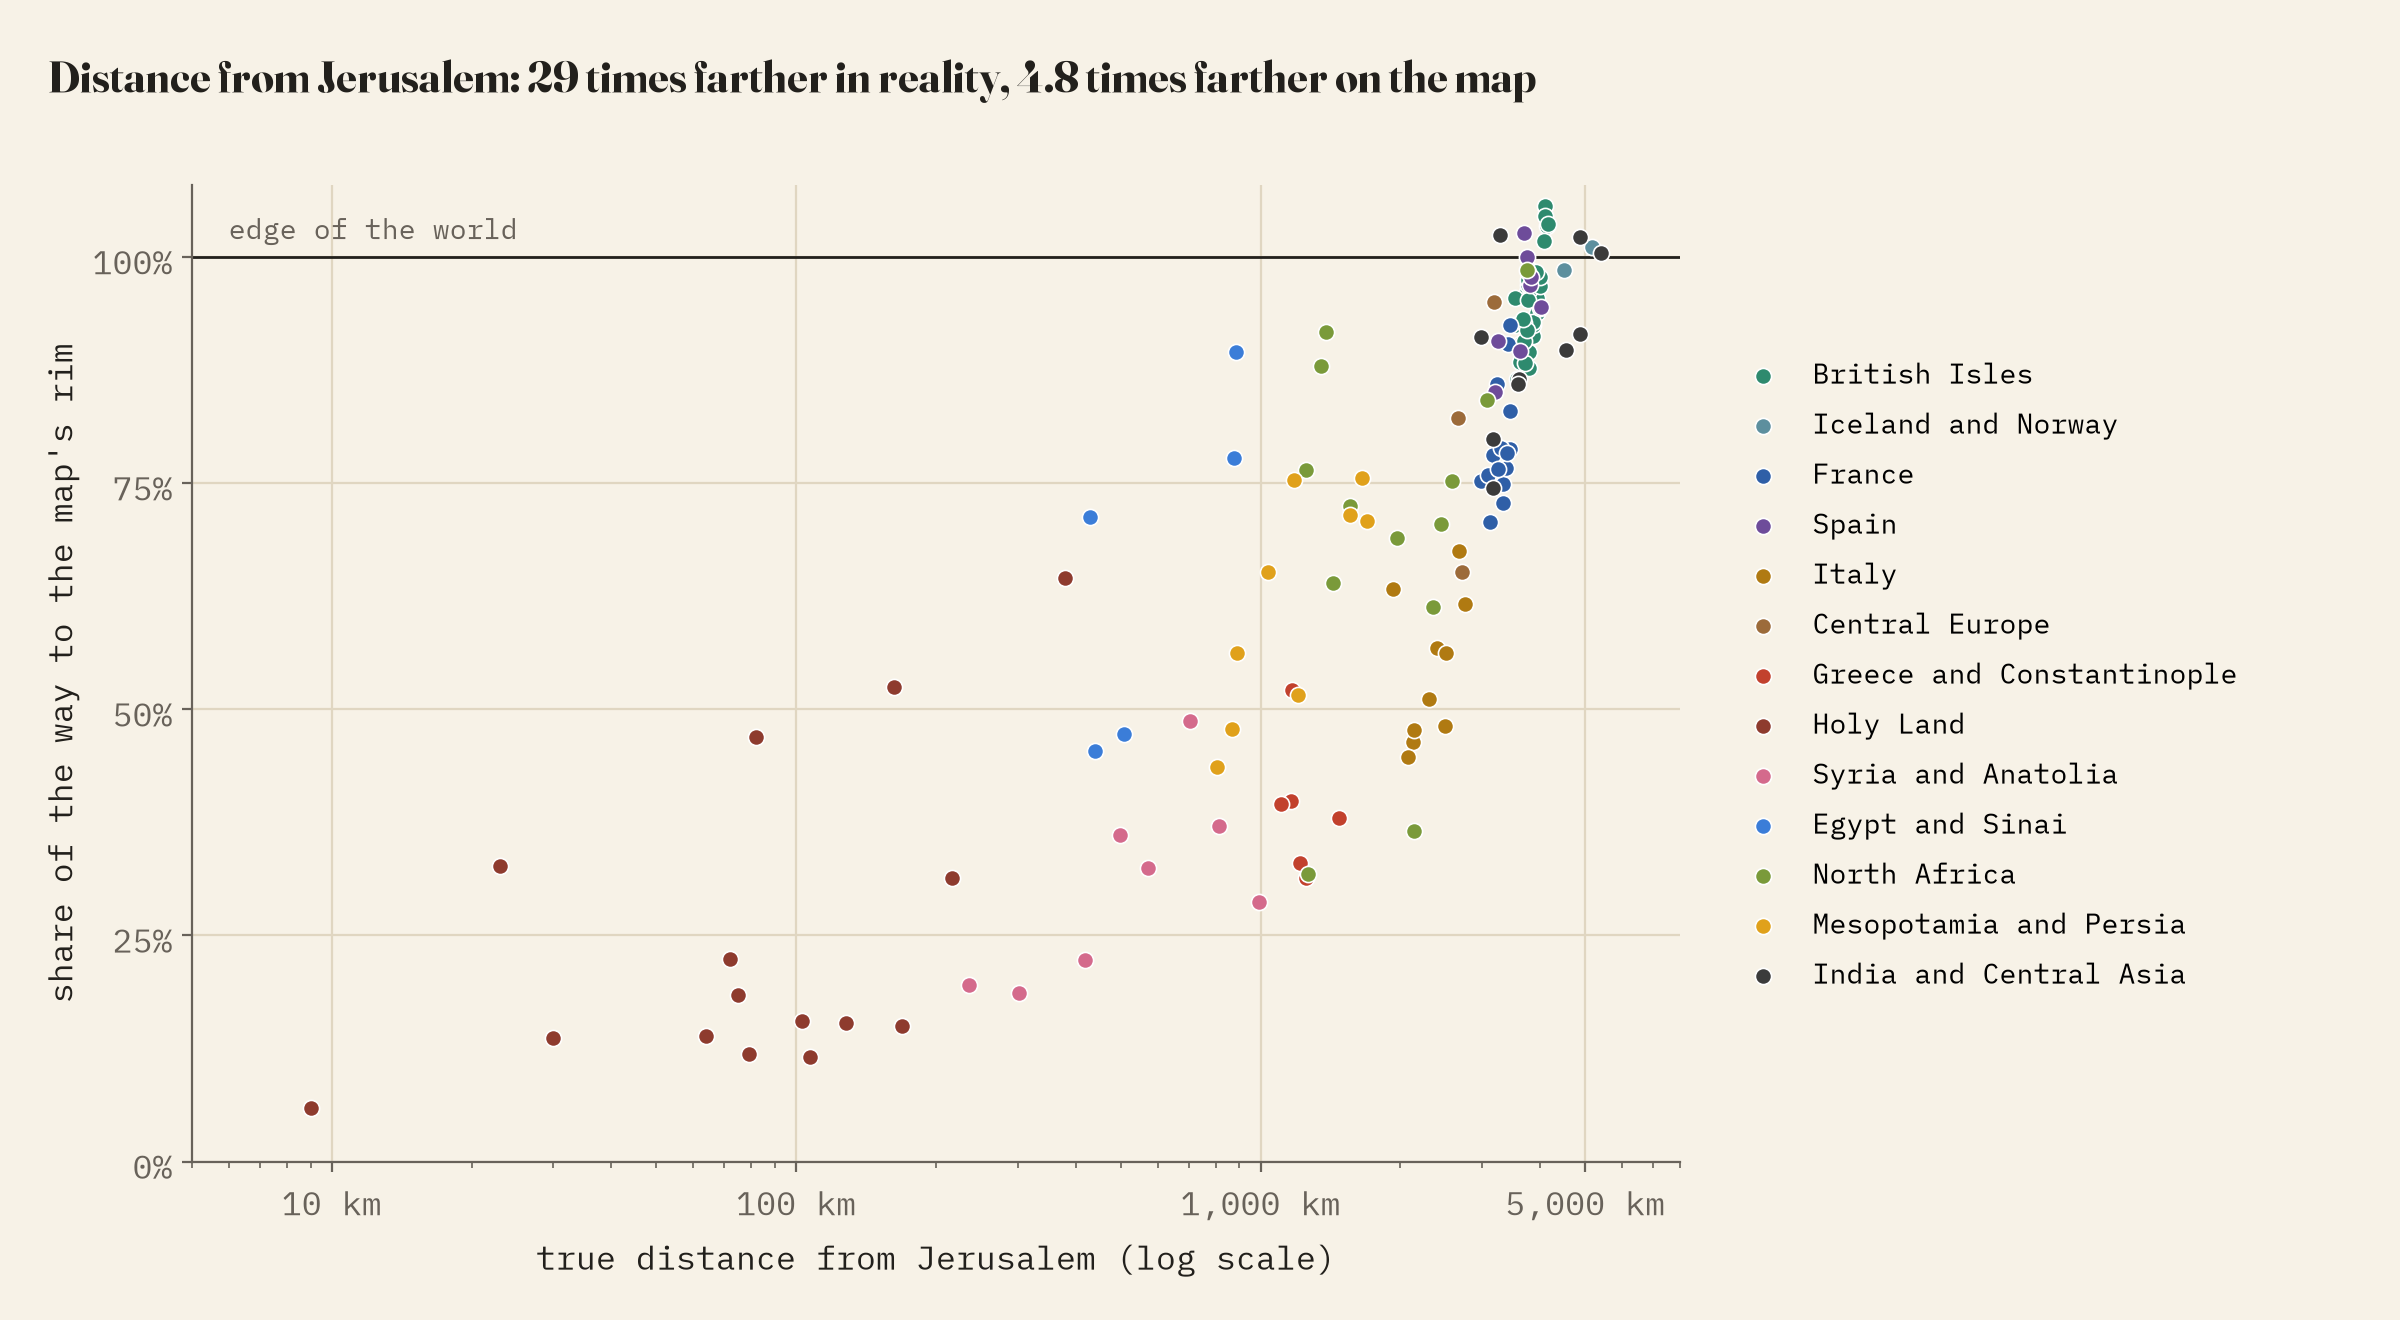
\includegraphics[width=\textwidth]{f_distance.png}
\caption{Distance from Jerusalem on the map, as a share of the way to the rim, against true distance (log scale).}\label{fig:distance}\end{figure}

\subsection{Scale by region}
Table~\ref{tab:regions} and Figure~\ref{fig:stretch} give the relative scale of each region. The Holy Land is drawn at 4.5 times the map's average, Egypt and Sinai at 1.9, Mesopotamia and Persia at 1.6, Syria and Anatolia at 1.5 and the British Isles at 1.5; Spain at 0.90 and India and Central Asia at 0.71. Iceland, the Faroes and Norway, too few to score, are squeezed into the rim.

\begin{table}[tbp]\centering\small\caption{Located real places by region: number, median true distance from Jerusalem, median distance on the map as a share of the radius, median absolute bearing error (degrees), relative scale, and median displacement from the best-fitting position (km).}\label{tab:regions}\begin{tabular}{lrrrrrr}\toprule Region & Places & km & Map & Error & Scale & Shift\\\midrule
British Isles & 35 & 3,801 & 96\% & 8 & 1.50 & 249\\
Iceland and Norway & 3 & 4,498 & 99\% & 12 & too few & 1,325\\
France & 15 & 3,325 & 78\% & 24 & 1.27 & 384\\
Spain & 8 & 3,717 & 96\% & 24 & 0.90 & 344\\
Italy & 10 & 2,352 & 54\% & 34 & 1.35 & 388\\
Central Europe & 3 & 2,720 & 82\% & 3 & too few & 804\\
Greece and Constantinople & 6 & 1,193 & 39\% & 8 & 1.29 & 884\\
Holy Land & 15 & 82 & 16\% & 50 & 4.55 & 776\\
Syria and Anatolia & 8 & 536 & 31\% & 28 & 1.53 & 1,062\\
Egypt and Sinai & 5 & 508 & 71\% & 72 & 1.86 & 973\\
North Africa & 13 & 1,970 & 72\% & 69 & 1.22 & 1,102\\
Mesopotamia and Persia & 9 & 1,183 & 65\% & 12 & 1.64 & 534\\
India and Central Asia & 10 & 3,594 & 90\% & 10 & 0.71 & 1,434\\
\bottomrule\end{tabular}\end{table}

\begin{figure}[tbp]\centering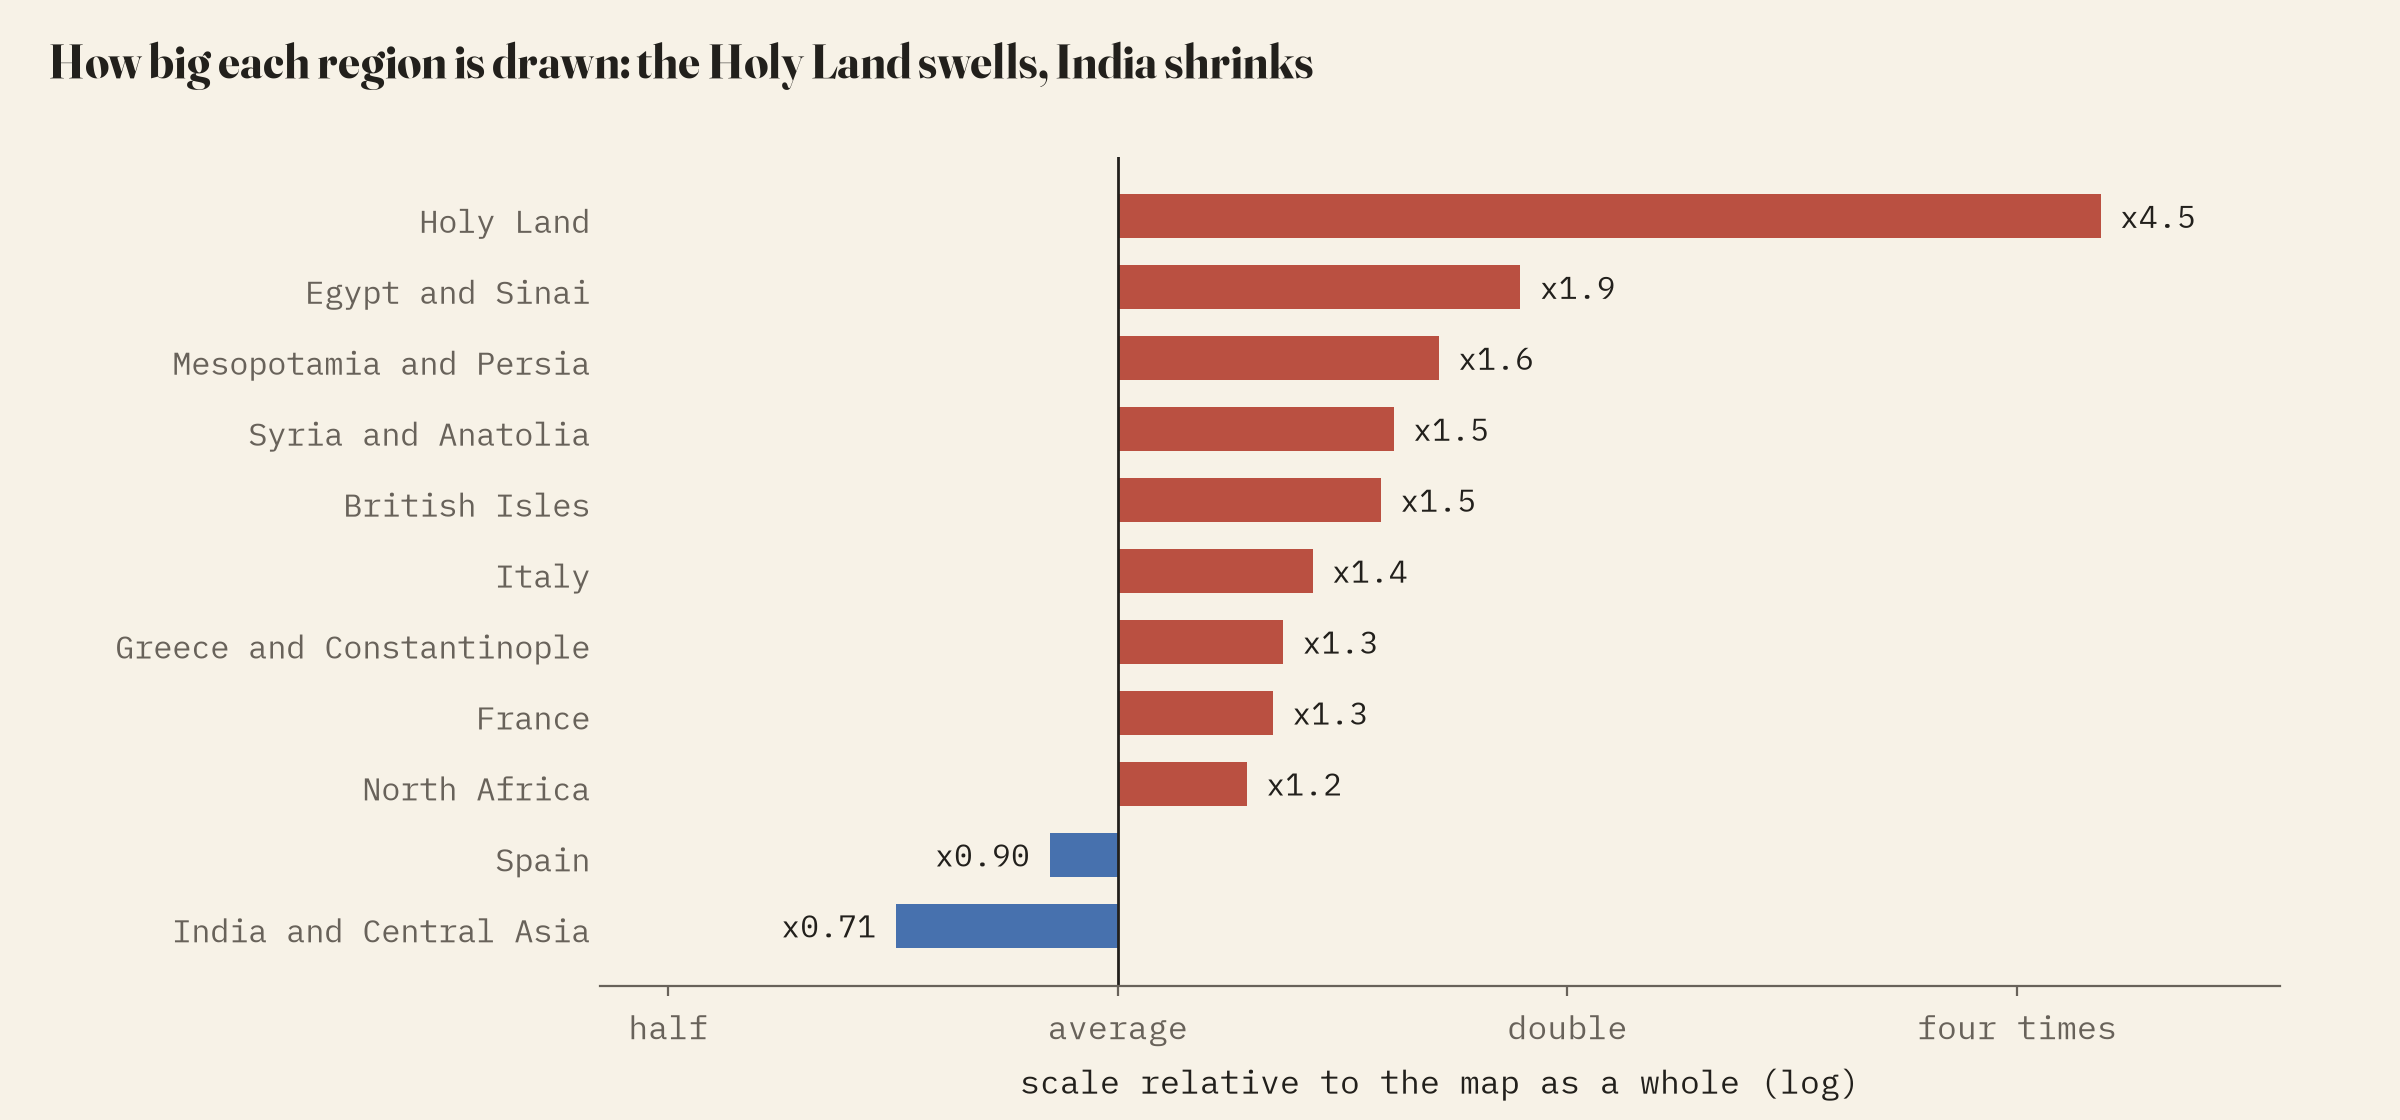
\includegraphics[width=\textwidth]{f_stretch.png}
\caption{Scale of each region relative to the map as a whole (median ratio of map to true distance over pairs of located places).}\label{fig:stretch}\end{figure}

\begin{figure}[tbp]\centering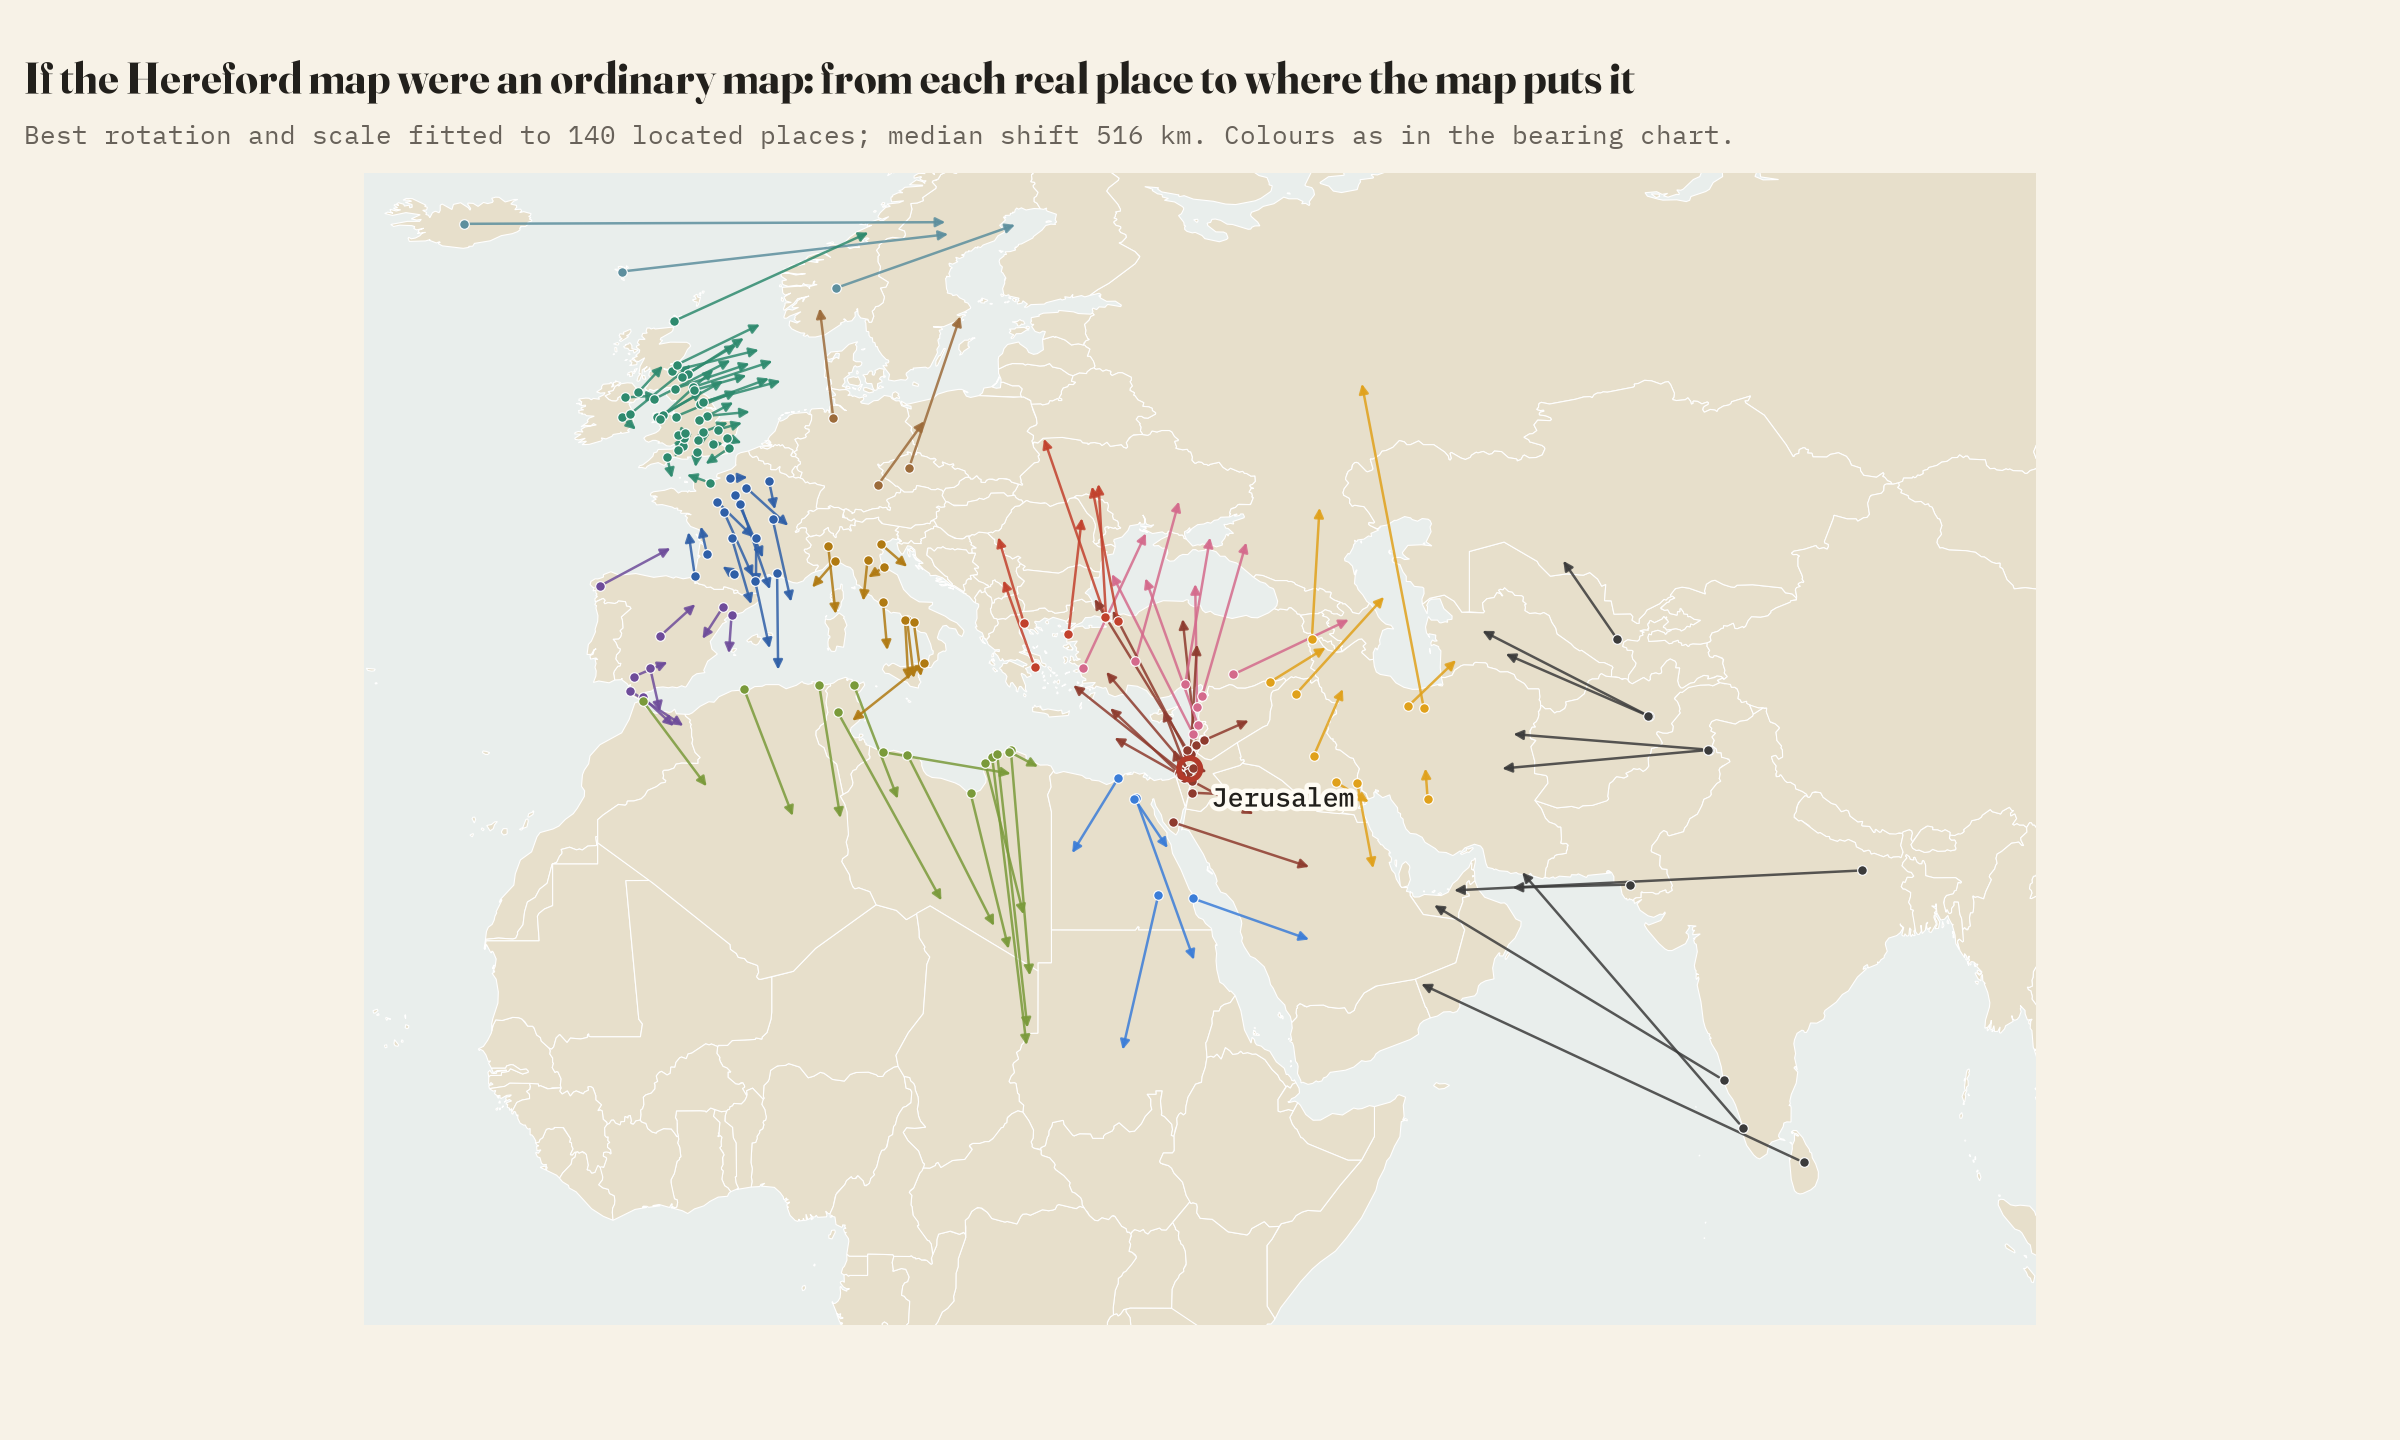
\includegraphics[width=\textwidth]{f_arrows.png}
\caption{Displacement of each located place from where the best-fitting rotation and scaling of the map would put it.}\label{fig:arrows}\end{figure}

\subsection{The British Isles}
The British Isles have 83 names, 8.1\% of the index, against 0.4\% of the land of Africa, Asia and Europe in Natural Earth's outlines, about 21 times their share. Bevan and Phillott judged them ``drawn on a scale out of all proportion to the other parts of the map'' and the rivers of the Humber depicted with ``a degree of accuracy which implies personal acquaintance''; they also noted gross errors, above all Caen, transferred ``by a strange blunder'' from Normandy to Devon \citep[pp. 163 to 170]{bevan}. Figure~\ref{fig:britain} compares the section with a modern map.

\begin{figure}[tbp]\centering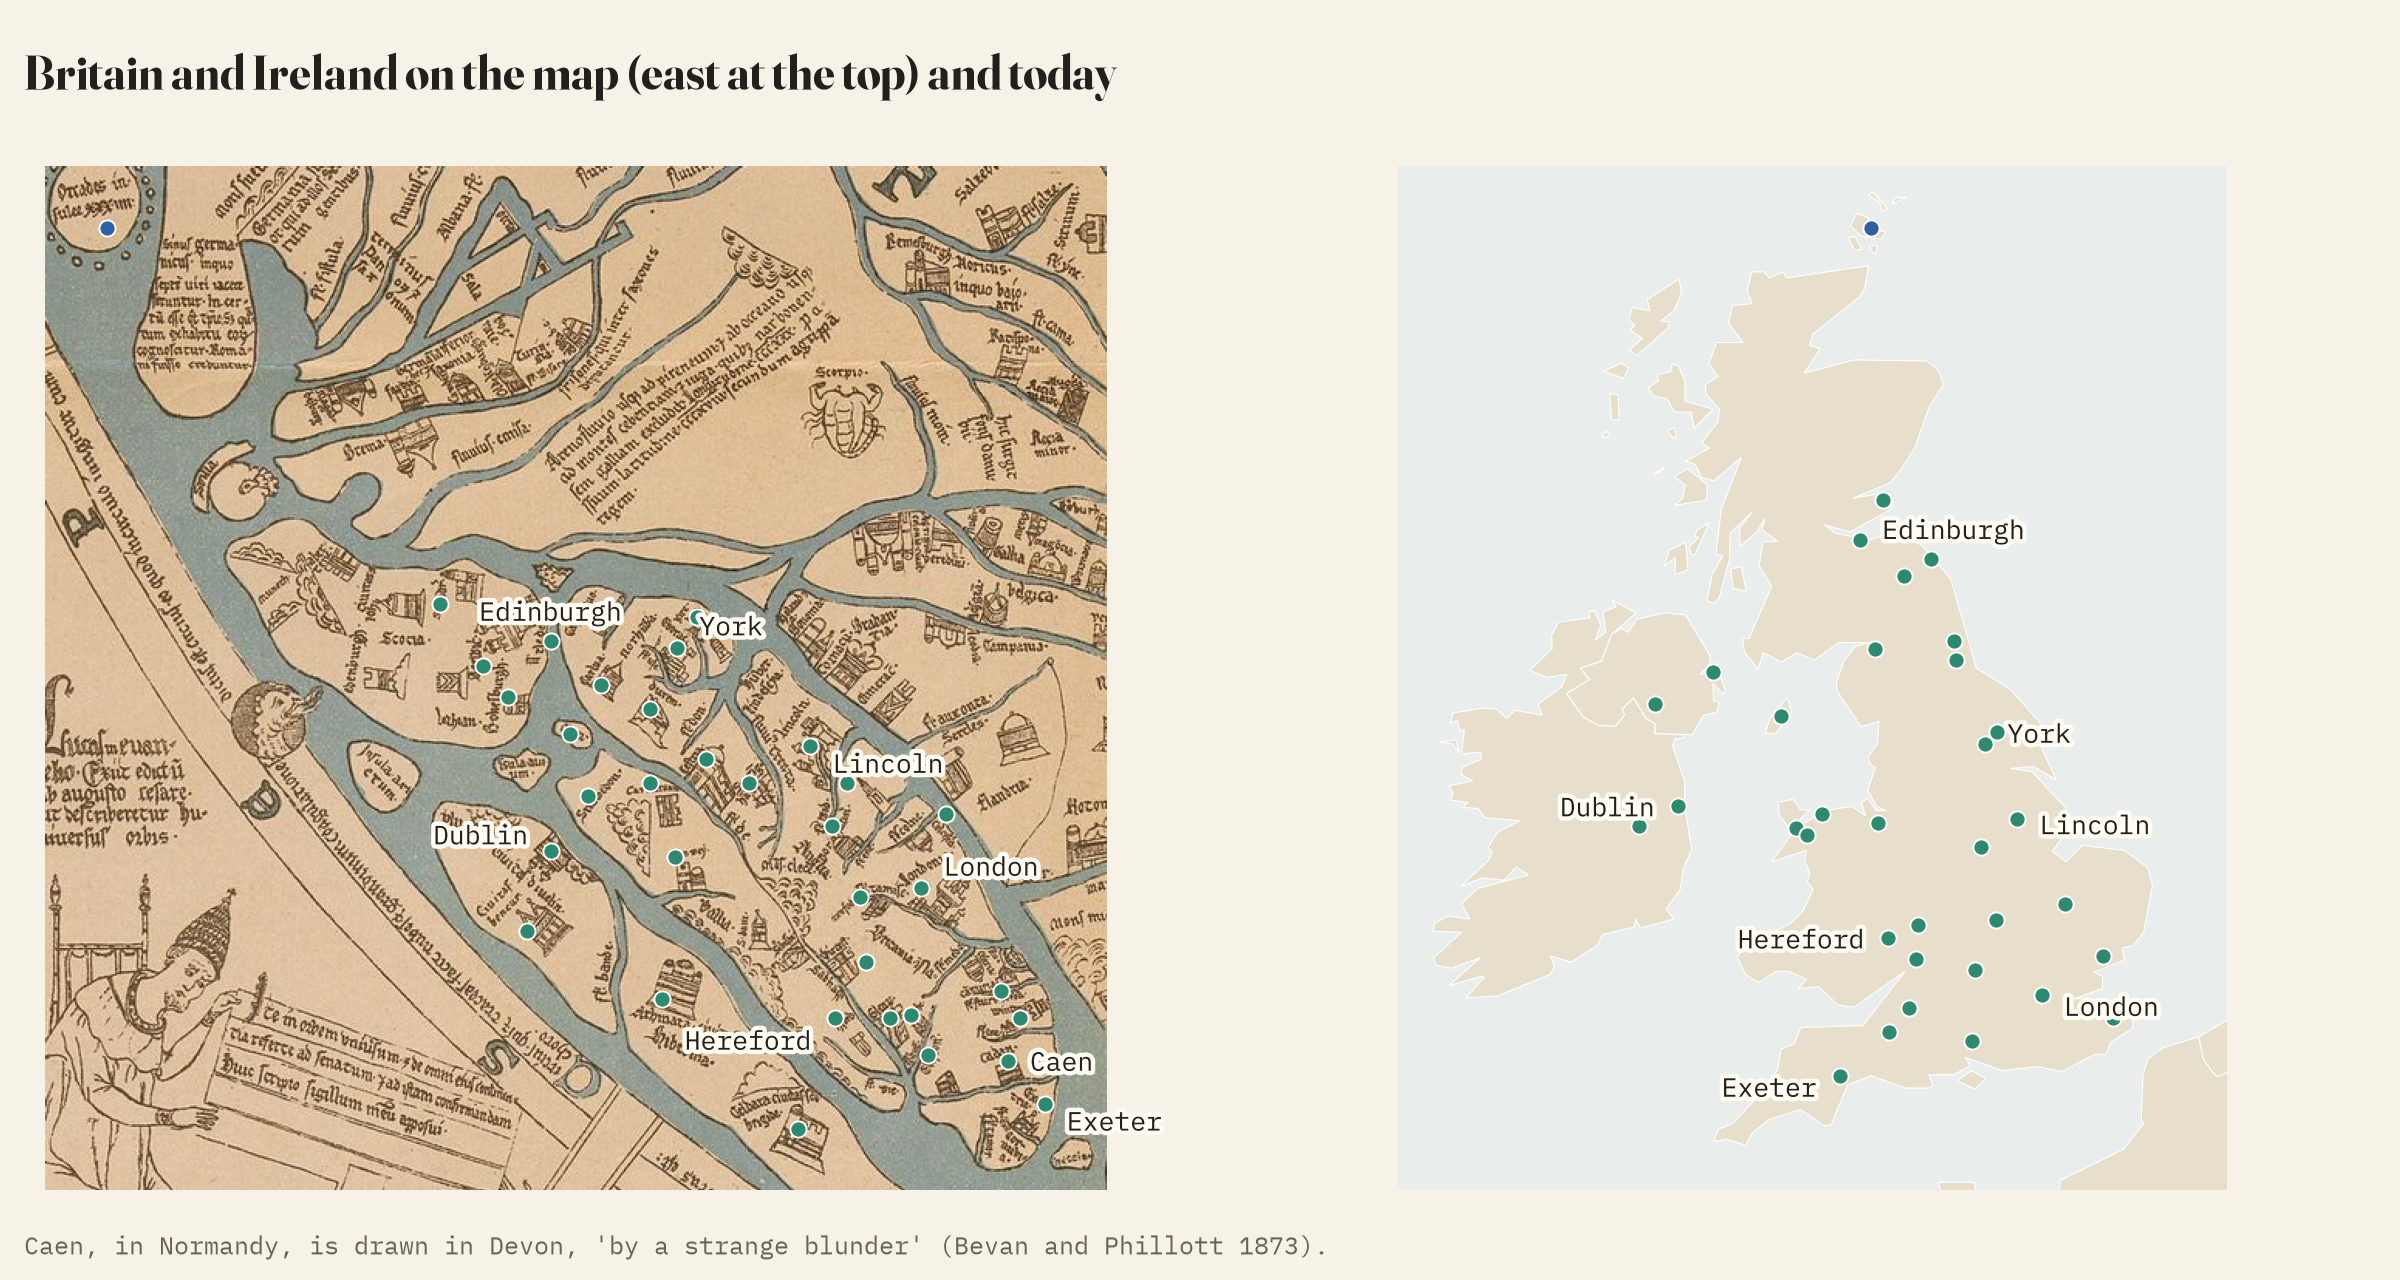
\includegraphics[width=\textwidth]{f_britain.png}
\caption{Britain and Ireland on the facsimile (east at the top) and today.}\label{fig:britain}\end{figure}

\section{Limitations}
First, the inventory is Bevan and Phillott's index, which records names, not pictures, and is not a complete modern edition; Westrem's edition and the Virtual Mappa project transcribe every inscription. Second, the classes rest on judgements made name by name, under a stated rule; others would draw some boundaries differently, especially between classical and medieval names in Europe. Third, the 1873 identifications are the Victorians' and some have been revised since; Pleiades matches by name are a lower bound on what can be identified. Fourth, positions were located by eye on a nineteenth century copy; the located set favours legible, well-known places, so the distortion figures describe the map's real towns rather than its whole surface. Fifth, the photograph is low resolution and the affine fit to it is approximate.

\section{Conclusion}
Measured against a modern map, the Hereford Mappa Mundi is not a failed attempt at geography but a different kind of map. Its directions from Jerusalem are mostly right once east is at the top, and its distances keep their order; what it gives up is scale, spending its space on the Holy Land, Egypt and Mesopotamia, where the Bible's history happened, and on the British Isles, where its makers lived, and pressing the rest of the world against the encircling ocean. Most of its names are inherited from late Roman books; the medieval present appears mainly at home.

\section*{Data and code availability}
The interactive comparison is at \url{https://maps.tristanhotham.com/mappa-mundi/}. Data and code are at \url{https://github.com/Tristan-Hotham/mappa-mundi} and archived with this paper at https://doi.org/10.5281/zenodo.23878612. Derived data are released under CC BY 4.0 and code under the MIT licence. The book and the map images are in the public domain; Pleiades data are CC BY 3.0.

\section*{AI statement}
I wrote the text, with drafting and editing assistance from Claude (Anthropic), which also helped prepare the analysis code. I reviewed and checked all text and results.

\begin{thebibliography}{9}
\bibitem[Bevan and Phillott(1873)]{bevan} Bevan, W. L. and Phillott, H. W. (1873) \textit{Mediaeval Geography: an Essay in Illustration of the Hereford Mappa Mundi}. London: E. Stanford. Internet Archive scan, public domain. \url{https://archive.org/details/medivalgeograph00unkngoog}
\bibitem[Miller(1896)]{miller1896} Miller, K. (1896) \textit{Richardi de Haldingham seu de Bello Mappamundi}, facsimile. Stuttgart: J. Roth. Wikimedia Commons, public domain. \url{https://commons.wikimedia.org/wiki/File:1896_facsimile_of_the_Hereford_Mappa_Mundi_by_Konrad_Miller.jpg}
\bibitem[Miller(1903)]{miller1903} Miller, K. (1903) \textit{Die Herefordkarte}. Stuttgart: J. Roth. Internet Archive scan, public domain. \url{https://archive.org/details/bub_gb_yJzVAAAAMAAJ}
\bibitem[Natural Earth(2026)]{naturalearth} Natural Earth (2026) Admin 0 countries and populated places, 1:50m and 1:10m. Public domain. \url{https://www.naturalearthdata.com/}
\bibitem[Pleiades(2026)]{pleiades} Bagnall, R. et al., eds. (2026) Pleiades: a gazetteer of past places, version 4.1. CC BY 3.0. \url{https://pleiades.stoa.org/}
\bibitem[Wikipedia(2026)]{wiki} Wikipedia contributors (2026) Hereford Mappa Mundi (revision 1381220355). CC BY-SA 4.0. \url{https://en.wikipedia.org/wiki/Hereford_Mappa_Mundi}
\end{thebibliography}

\clearpage
\appendix
\section{The located inscriptions}
{\footnotesize\setlength{\tabcolsep}{4pt}\begin{longtable}{p{3.2cm}rlp{6.6cm}l}\caption{The 164 inscriptions located on Miller's facsimile, with the 1873 book's page, the class, the identification and my confidence in the position.}\label{tab:located}\\\toprule Name (index) & Page & Class & Identification (Bevan and Phillott) & Position\\\midrule\endfirsthead\toprule Name (index) & Page & Class & Identification & Position\\\midrule\endhead
Apollonia & 92 & Classical & Apollonia (Susa, Libya) & high\\
Aree Philenoram & 92 & Classical & the Altars of the Philaeni & high\\
Arsinoe & 92 & Classical & Arsinoe (Tocra, Teuchira) & high\\
Berenice & 92 & Classical & Benghazi (Berenice) & high\\
Blemee & 103 & Legendary & (no real place) & medium\\
Calpel & 99 & Classical & Gibraltar (Calpe) & high\\
Cartago & 95 & Classical & Carthage & high\\
Cesarea & 99 & Classical & Caesarea in Mauretania (Cherchell) & medium\\
Cirene & 92 & Classical & Cyrene (Shahhat) & high\\
Fortunate & 106 & Legendary & (no real place) & medium\\
Ippone & 97 & Classical & Hippo Regius (Annaba) & high\\
Leptis Magna & 93 & Classical & Leptis Magna & high\\
Ptholomaida & 92 & Classical & Ptolemais (Tolmeita) & high\\
Sabrata & 93 & Classical & Sabratha & medium\\
Scinopodes & 102 & Legendary & (no real place) & high\\
Septem Montes & 99 & Classical & Ceuta & high\\
Suffetula & 96 & Classical & Sufetula (Sbeitla) & high\\
Alexandria & 88 & Classical & Alexandria & high\\
Alexandria & 36 & Classical & Alexandria in the Caucasus (Bagram) & medium\\
Antiochia & 68 & Classical & Antioch in Pisidia & medium\\
Antiochia & 76 & Classical & Antioch of Syria (Antakya) & high\\
Arbor Sicca & 25 & Legendary & (no real place) & medium\\
Area Noe & 69 & Biblical & the mountains of Armenia (Ararat) & high\\
Aree Alexandri & 28 & Classical & (no real place) & high\\
Ascalon & 78 & Biblical & Ashkelon & high\\
Avalerion & 30 & Legendary & (no real place) & high\\
Babel Tttkris & 74 & Biblical & Babylon (the Tower of Babel) & high\\
Babylonia & 74 & Biblical & Babylon & medium\\
Babylonia & 86 & Classical & Cairo & high\\
Berenice & 84 & Classical & Berenice on the Red Sea & medium\\
Beritus & 76 & Classical & Beirut & high\\
Bersabee & 80 & Biblical & Beersheba & high\\
Bethleem & 79 & Biblical & Bethlehem & high\\
Bucephala & 28 & Classical & Bucephala on the Hydaspes (Jhelum) & medium\\
Calcidonia & 69 & Classical & Chalcedon (Kadikoy) & medium\\
Carax & 72 & Classical & Charax Spasinou & high\\
Carimaspi & 61 & Legendary & (no real place) & medium\\
Carmelum & 78 & Biblical & Mount Carmel & medium\\
Caspia & 52 & Classical & (no real place) & high\\
Caspie Portee & 64 & Classical & the Caspian Gates & high\\
Cassica & 30 & Classical & Capissa (Kapisa) & medium\\
Cesarea Philippi & 78 & Biblical & Caesarea Philippi (Banias) & high\\
Cottonare & 27 & Classical & Kochi (Cochin) & medium\\
Damascus & 77 & Biblical & Damascus & high\\
Ebron & 80 & Biblical & Hebron & medium\\
Enos & 27 & Biblical & (no real place) & high\\
Ephesus & 68 & Classical & Ephesus & high\\
Gaza & 79 & Biblical & Gaza & high\\
Gerara & 79 & Biblical & Gerar & high\\
Gigantes & 27 & Legendary & (no real place) & high\\
Griphe & 61 & Legendary & (no real place) & high\\
Hur & 74 & Biblical & Ur of the Chaldees & high\\
Jerico & 80 & Biblical & Jericho & medium\\
Jerusalem & 79 & Biblical & Jerusalem & high\\
Laodiciam & 76 & Classical & Latakia (Laodicea of Syria) & high\\
Loth uxor & 77 & Biblical & (no real place) & high\\
Magog & 49 & Legendary & (no real place) & medium\\
Mandragora & 87 & Frame & (no real place) & high\\
Nazaret & 78 & Biblical & Nazareth & high\\
Nicea & 28 & Classical & Nicaea on the Hydaspes (Jhelum) & medium\\
Nicomedia & 69 & Classical & Nicomedia (Izmit) & medium\\
Ninevee & 73 & Biblical & Nineveh (Mosul) & high\\
Nisibi & 74 & Classical & Nisibis (Nusaybin) & high\\
Orrea Josepbi & 86 & Biblical & the Pyramids of Giza & high\\
Paradisi porte & 25 & Legendary & (no real place) & high\\
Patalus & 28 & Classical & the Indus delta (Patale) & medium\\
Persepolis & 72 & Classical & Persepolis & high\\
Petra & 77 & Classical & Petra & medium\\
Phenix & 85 & Legendary & (no real place) & high\\
Pigmei & 28 & Legendary & (no real place) & high\\
Polibrota & 32 & Classical & Patna (Palimbothra) & high\\
Rages & 71 & Classical & Rhagae (Rey, Tehran) & high\\
Samarcan & 52 & Medieval & Samarkand & high\\
Samosaka & 73 & Classical & Samosata & high\\
Siene & 84 & Classical & Aswan (Syene) & high\\
Sinay & 81 & Biblical & Mount Sinai & high\\
Sodom & 77 & Biblical & Sodom, by the Dead Sea & medium\\
Tapbana & 34 & Classical & Sri Lanka (Taprobane, Ceylon) & high\\
Tarsus & 68 & Classical & Tarsus & high\\
Tholomaida & 78 & Biblical & Acre (Ptolemais) & high\\
Tripolis & 76 & Classical & Tripoli, Lebanon & high\\
Troja & 69 & Classical & Troy & medium\\
Zimarim & 33 & Classical & Muziris, now probably Mangalore & high\\
Arhmata & 172 & Medieval & Armagh & high\\
Bathe & 170 & Medieval & Bath & medium\\
Bencur & 172 & Medieval & Bangor, County Down & medium\\
Berwic & 171 & Medieval & Berwick-upon-Tweed & high\\
Cadan & 170 & Medieval & Caen (misplaced in England) & high\\
Canturia & 170 & Medieval & Canterbury & medium\\
Carlua & 169 & Medieval & Carlisle & high\\
Carnarvan & 171 & Medieval & Caernarfon & high\\
Castello Novo & 169 & Medieval & Newcastle upon Tyne & medium\\
Celdara & 172 & Medieval & Kildare & high\\
Cestria & 169 & Medieval & Chester & high\\
Colcestria & 168 & Medieval & Colchester & high\\
Cunwey & 171 & Medieval & Conwy & high\\
Divelin & 172 & Medieval & Dublin & medium\\
Durem & 169 & Medieval & Durham & high\\
Eboracum & 169 & Medieval & York & high\\
Edenburgh & 171 & Medieval & Edinburgh & medium\\
Ely & 168 & Medieval & Ely & high\\
Excestria & 170 & Medieval & Exeter & medium\\
Glearum & 169 & Medieval & Gloucester & medium\\
Glestonia & 170 & Medieval & Glastonbury & medium\\
Hreford & 169 & Medieval & Hereford & high\\
Kircham & 169 & Medieval & Kirkham Priory & medium\\
Lincoln & 168 & Medieval & Lincoln & high\\
Londonia & 168 & Medieval & London & high\\
Man & 172 & Medieval & the Isle of Man & high\\
Norhanton & 168 & Medieval & Northampton & medium\\
Oxeford & 168 & Medieval & Oxford & high\\
Rokesburg & 171 & Medieval & Roxburgh & high\\
S. Andr & 171 & Medieval & St Andrews & high\\
Snawedon & 171 & Medieval & Snowdon & high\\
Snotingham & 169 & Medieval & Nottingham & high\\
Wintona & 170 & Medieval & Winchester & high\\
Wircestr & 169 & Medieval & Worcester & medium\\
Arelas & 148 & Classical & Arles & high\\
Arimmuin & 130 & Classical & Rimini & medium\\
Athene & 134 & Classical & Athens & medium\\
Augustudunum & 145 & Classical & Autun & medium\\
Aurelianum & 146 & Classical & Orleans & medium\\
Avernis & 147 & Classical & Clermont-Ferrand & high\\
Basella & 126 & Medieval & Seville & high\\
Bayona & 148 & Medieval & Bayonne & high\\
Bononia & 130 & Classical & Bologna & high\\
Braga & 152 & Classical & Prague & high\\
Brema & 152 & Medieval & Bremen & high\\
Burdegala & 147 & Classical & Bordeaux & medium\\
Carnotum & 146 & Classical & Chartres & high\\
Cenomani & 146 & Classical & Le Mans & high\\
Cinocephales & 159 & Legendary & (no real place) & high\\
Compostella & 125 & Medieval & Santiago de Compostela & high\\
Constantinopolis & 136 & Classical & Istanbul (Constantinople) & high\\
Corduba & 126 & Classical & Cordoba & high\\
Fareie & 162 & Medieval & the Faroe Islands & high\\
Ganzmir & 158 & Legendary & (no real place) & high\\
Genua & 131 & Classical & Genoa & medium\\
Iacobi Templum & 125 & Medieval & Santiago de Compostela (the shrine of St James) & high\\
Ilerda & 126 & Classical & Lleida (Lerida) & high\\
Limogena & 147 & Classical & Limoges & high\\
Narbona & 143 & Classical & Narbonne & high\\
Neapolis & 131 & Classical & Naples & high\\
Noreya & 158 & Classical & Norway & high\\
Orcades & 161 & Classical & Orkney & high\\
Parisius & 145 & Classical & Paris & high\\
Puteolis & 131 & Classical & Pozzuoli & high\\
Remesburgh & 154 & Medieval & Regensburg & high\\
Remis & 145 & Classical & Reims & high\\
Roma & 130 & Classical & Rome & high\\
Rotomagum & 145 & Classical & Rouen & high\\
Salema & 131 & Classical & Salerno & high\\
Terracona & 126 & Classical & Tarragona & high\\
Thessalonica & 135 & Classical & Thessaloniki & high\\
Toletum & 126 & Classical & Toledo & high\\
Tolosa & 147 & Classical & Toulouse & medium\\
Turonis & 147 & Classical & Tours & medium\\
Vercellis & 130 & Classical & Vercelli & medium\\
Ysland & 162 & Medieval & Iceland & high\\
Caribdis & 116 & Legendary & (no real place) & high\\
Gades & 112 & Classical & Cadiz & high\\
Laborintus & 116 & Legendary & (no real place) & high\\
Messana & 116 & Classical & Messina & high\\
Venicia & 118 & Classical & Venice & high\\
\bottomrule\end{longtable}}
\end{document}
